\section{Motivating example}

The crux of the trace forensics problem is: How can we provide hints of proximal causes when an execution fails? \ash{We should proximal cause in the introduction section as well, if we want to use it here.}

\begin{figure}[h]
\center{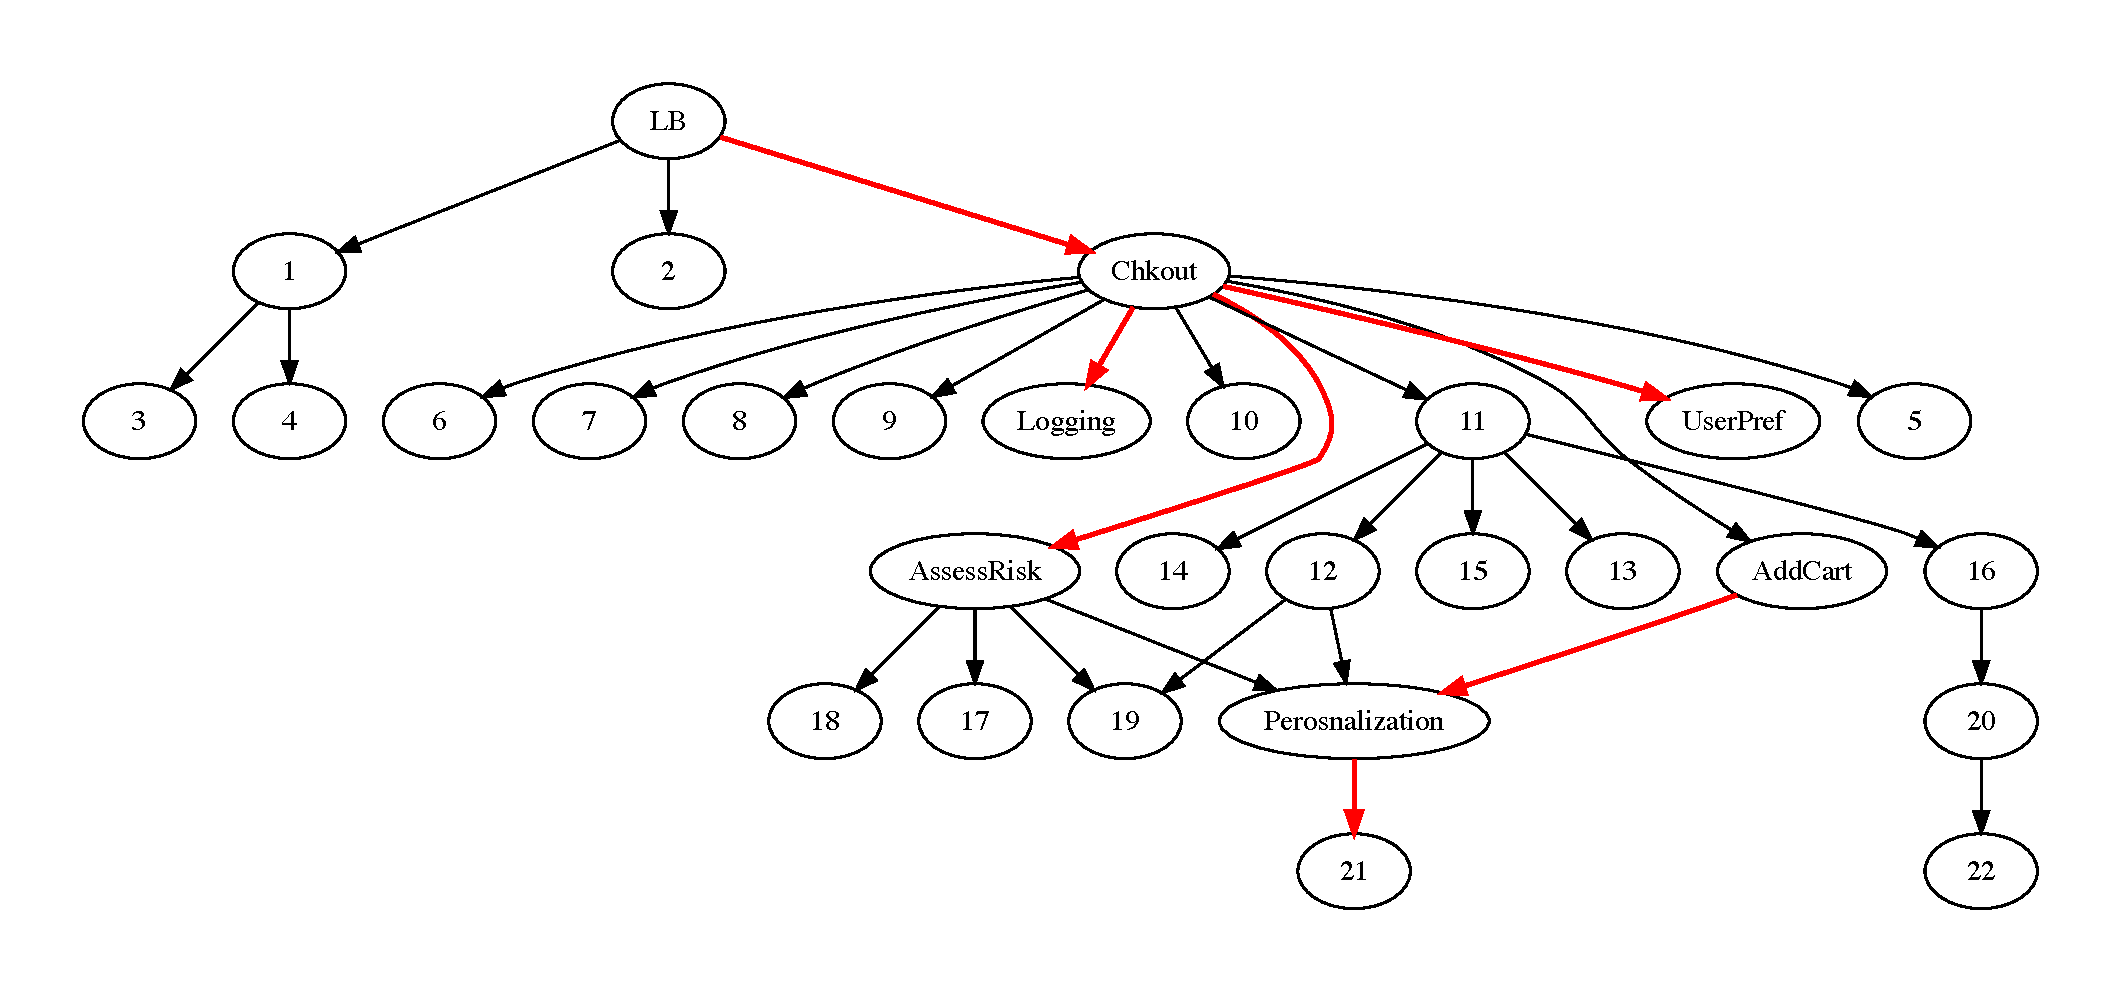
\includegraphics[scale=0.25]{anon_adrbk_fail.pdf}}
\caption{Example graph drawn from trace of a failed interaction. The red lines indicate that the callee has returned an error message to the caller}
\label{Failed_ex}
\end{figure}

Figure~\ref{Failed_ex} shows the  call-graph of a user interaction involving checkout of items for a cart, which ultimately fails. 
A successful checkout occurs when the user is able to place an order, else the checkout fails. 
When failures are observed, it is the job of a site reliability engineer (SRE) to troubleshoot the failure. 
Currently, the SRE sees a number of alerts \ash{arising from failures, possibly in rpc calls highligted as red in the call graph,} from the monitoring system that maintains aggregate data over sliding windows of time for all services.
\ash{I don't think the second half of this sentence is true in general. We should probably look to re-phrase it.} 
The SRE might go about their job like so:
\begin{itemize}
\item Figure out which of the alerts are smokescreens to be ignored. \newline
Some services that are called as part of the interaction which provide useful functionality, but the failure of which can be tolerated by the system. 
These can be thought of as nice-to-have \ash{soft dependencies} services. Alerts from such services may be safely ignored and an SRE would generally be able to identify these with experience.
\ash{One can argue that the alerts should be suppressed and never be raised.}
\item Use domain knowledge about the dependencies between services to know which alerts are the result of transitive dependencies and must be ignored. \newline
As an example, the load balancer (LB) in the figure will be alerting. 
An intelligent \ash{let's leave out the intelligent bit} SRE would conclude that since checkout (Chkout) has multiple downstream alerts, the alerts at LB are probably a result of the error being propagated up and try to dig deeper into one of the downstream alerts that look promising \ash{promising for ? proximal cause I assume}. 
Once a promising alert has been found, it is now time to look at the logs from the appropriate time to try to determine cause of failure.
\item Determine if the absence \ash{loose word.. do you mean failure ?}of some service(s) caused the failure \newline
Failures are sometimes caused by failure of mandatory services or a fallback path not being taken. Details of a network connection failure or time out in attempting to connect to downstream services might be buried deep in the logs, taking longer to unearth and fix, resulting in larger user downtimes. 
\end{itemize}

\ash{We went from SRE triage process to, describing the sections of our paper. This felt very jumpy. We need a closing argument. The motivation didn't come through. We didn't say why the life of the SREs is difficult give these steps? And how we will potentially solve the problems.}
In the next section, we describe the generation of trace embeddings and the corresponding distance measure used. 
In the evaluation, we describe how we use the fairly simple operations on the embeddings to address the problem described above and automatically generate hints about the proximal causes for the failure observed. 
This is made possible due to the fact that the embeddings encode information of structural neighborhoods.
